\section{Scene Surveying With Heterogeneous Battery Constraints and Sampling Times}
\note{Keep this very brief - there is not a great research output here. Simply mention that we began looking into using solvers to calculate solutions as is line with a lot of the literature.}

Once we had prototyped the NN algorithm in order to find a suitable solution to the simplified problem, we then considered the more general problem, where RAVs have heterogeneous battery constraints, sampling times and operational speeds, which is mentioned in section \ref{sec:SceneSurveying}. This can be described by the more general Vehicle Routing Problem (VRP). We decided to formulate the problem as a \textit{linear program} and planned to find solutions using a linear program solver, following the literature outlined in section <reference>. We subsequently use terminology commonly used in convex optimisation and linear programming. We refer the reader to the text "Convex Optimization" \cite{Boyd2004ConvexOptimization} for information on linear programming and convex optimisation in general. This means that the problem's objective function and constraints must be written as linear expressions.
%A number of code repositories with permissive licences that provide solvers for linear programs exist .S
Specifying the VRP explicitly as a linear program and then passing it to a solver is a time-consuming process, which has led to the development of a number of tools which act as wrappers for software developers to solve well-known problems without having to write excessive amounts of boiler-plate code. We chose to use Google's Apache-licensed \href{https://developers.google.com/optimization/}{\textit{Operations Research}}\footnote{\href {https://developers.google.com/optimization/}{https://developers.google.com/optimization/}} (OR) repository, which contains a routing library with high-level interfaces specifically designed to allow the user to define and solve VRPs. This meant we could focus on defining the salient aspects of the problem rather than the details of how to convert the VRP into a linear program.

We began by following the example outlined in the \href{https://developers.google.com/optimization/routing/vrp}{OR tools documentation}\footnote{\href {https://developers.google.com/optimization/routing/vrp}{https://developers.google.com/optimization/routing/vrp}}. The documentation outlines the steps to solve a linear program using the repo follow the same pattern: 
\begin{itemize}
\item Create the variables.
\item Define the constraints.
\item Define the objective function.
\item Declare the solver — the method that implements an algorithm for finding the optimal solution.
\item Invoke the solver and display the results.
\end{itemize}

In order to follow these steps, we added the following to the provided example code:

\subsection{Specifying Variables and Constraints}
We first implemented a vehicle class which records the variables related to routing for each vehicle. Member variables included:
\begin{itemize}
    \item The time taken to record data at each node
    \item The location of the depot, where the charging point is located
    \item The operational speed of the vehicle
    \item The estimated remaining battery life in seconds
\end{itemize}
In order to facilitate recharging, we followed the approach outlined in the documented examples and created "virtual" depot nodes, which are duplicate nodes of the recharge location and have an associated recharge time for each RAV.  We force the RAVs to visit the depot to recharge once its battery level reaches below 5\% by creating a cumulative variable with a range equal to the predicted time taken for the RAV battery to degrade to this level. In effect, this indicates to the solver that it must include a virtual depot node in the solution at this time.

For each RAV, we then created a lookup table of times taken to travel from one node to the next and service the second node, based on the distances between the nodes, the operational speed of the RAV and the service time. In order to communicate to the solver that it should refer to each of these lookup tables to determine the cost of adding a node to a vehicle's route, we created a \textit{dimension} for each vehicle which refers to the lookup table. \textit{Dimensions} are used in the OR Tools interface to represent quantities accumulated at nodes along the routes. We then specified each time dimension to contribute to the objective function by using the setGlobalSpanCostCoefficient method, which notifies the solver to minimise the largest cost among all the time dimensions, which equates to minimising the longest time taken for any vehicle to complete its route. Since the solver is designed to find solutions to mixed-integer linear programs, we took the recommended approach of scaling up distance between nodes and then rounding, in order to minimise error. Once the solution had been computed, we normalised the results to their original scale. We used the default CP-SAT solver to compute a solution, with the cheapest arc heuristic. The cheapest arc heuristic builds a solution by beginning with the start node and connects it to the node which produces the cheapest route segment, then extends the route by iterating on the last node added to the route. We did not get the chance to evaluate other heuristics due to time constraints.

\subsection{Results of the Solver-Based Method}

Due to time constraints, we only managed to prototype the OR-Tools solver based method, which meant the results that we generated apply to carefully chosen regions that offer a proof-of-concept that the OR-Tools based method can provide viable solutions. We outline in section \ref{sec:SurveyingConclusionFutureWork} how we envision the prototype solution could be extended and sufficiently validated. Sample solutions computed for various configurations of the vehicles are shown in Table \ref{table:ORToolsResults}. For each of the solutions shown, we enforced that RAV 1 (red) and RAV 2 (green) have 1200 seconds fly time and that RAV 3 (yellow) has 2400 seconds of flying time. We assumed arbitrarily that the RAVs take 600 seconds to recharge to full capacity and that the RAVs will always recharge to full capacity if they return to the depot node. RAV 1, RAV 2 and RAV 3 begin with 17.5\%, 33.3\% and 100\% of their full battery capacities respectively. RAVs start and finish at the same location.

The configurations and solutions for the individual vehicles used are given in Table \ref{table:ORToolsResults}
\note{Ran with 3 RAVs also, might be worth showing}
\begin{table}[h!]
  \centering
  \begin{tabular}{ | c | m{5.2cm} | }
    \hline
    Planned RAV Routes & Solution details \\
    \hline
    
    %single RAV
    \begin{minipage}[c][53mm][c]{.6\textwidth}
      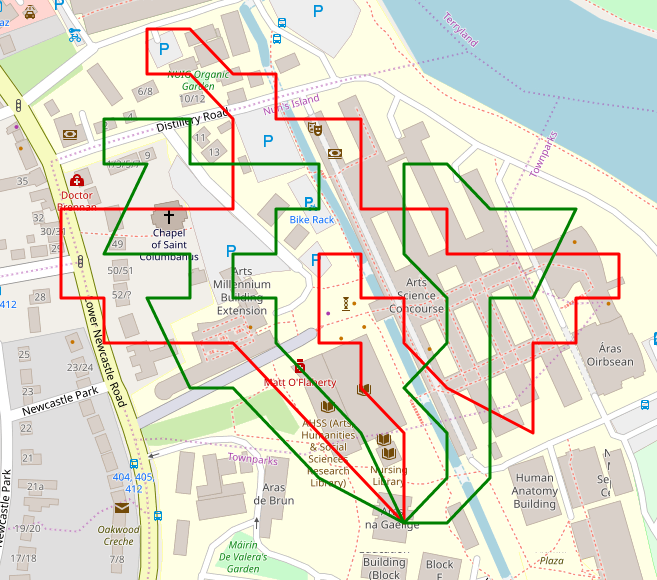
\includegraphics[width=\linewidth, height=51mm]{Chapters/MultiAgentCoverage/MultipleTravellingSalesman/Figs/ORToolsSolns/Example1.PNG}

    \end{minipage}
    &
    \small
    \begin{tabular}{m{10mm}|m{11mm} m{11mm}}
        & RAV 1 & RAV 2\\
        \hline
        Speed& 4 & 2 \\
        T.T.S & 0.5 & 0.5 \\
        Color & Red & Green \\
        \hline
        Dist.& 1813 & 1813 \\
        Time& 1410 & 1600 \\
    \end{tabular}
    \normalsize
    \\
    \hline
    %single RAV
    \begin{minipage}[c][53mm][c]{.6\textwidth}
      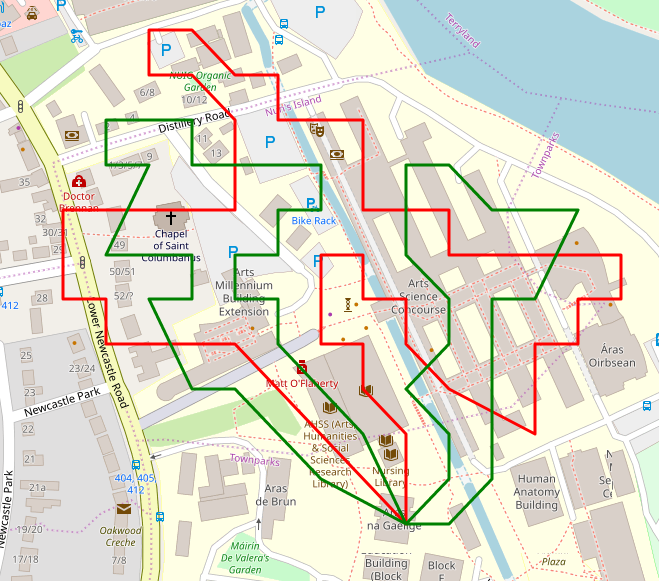
\includegraphics[width=\linewidth, height=51mm]{Chapters/MultiAgentCoverage/MultipleTravellingSalesman/Figs/ORToolsSolns/Example2.PNG}

    \end{minipage}
    &
    \small
    \begin{tabular}{m{10mm}|m{11mm} m{11mm} }
        & RAV 1 & RAV 2\\
        \hline
        Speed& 1 & 1 \\
        T.T.S & 0.5 & 0.5 \\
        Color & Red & Green \\
        \hline
        Dist.& 1961 & 2141 \\
        Time& 3423 & 3423 \\
    \end{tabular}
    \normalsize
    \\
    \hline
    
    %single RAV
    \begin{minipage}[c][53mm][c]{.6\textwidth}
      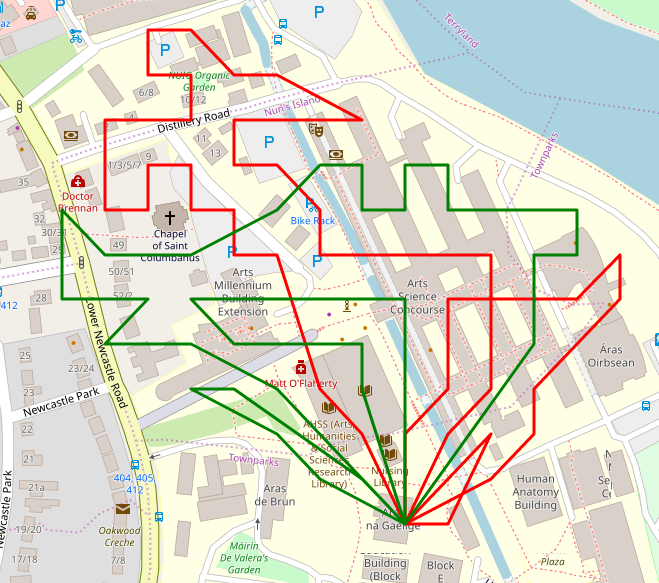
\includegraphics[width=\linewidth, height=51mm]{Chapters/MultiAgentCoverage/MultipleTravellingSalesman/Figs/ORToolsSolns/Example3.PNG}

    \end{minipage}
    &
    \small
    \begin{tabular}{m{10mm}|m{11mm} m{11mm}}
        & RAV 1 & RAV 2\\
        \hline
        Speed& 1 & 1 \\
        T.T.S & 2 & 2 \\
        Color & Red & Green \\
        \hline
        Dist.& 2142 & 2150 \\
        Time& 3462 & 3462 \\
    \end{tabular}
    \normalsize
    \\
    \hline
    
    %single RAV
    \begin{minipage}[c][53mm][c]{.6\textwidth}
      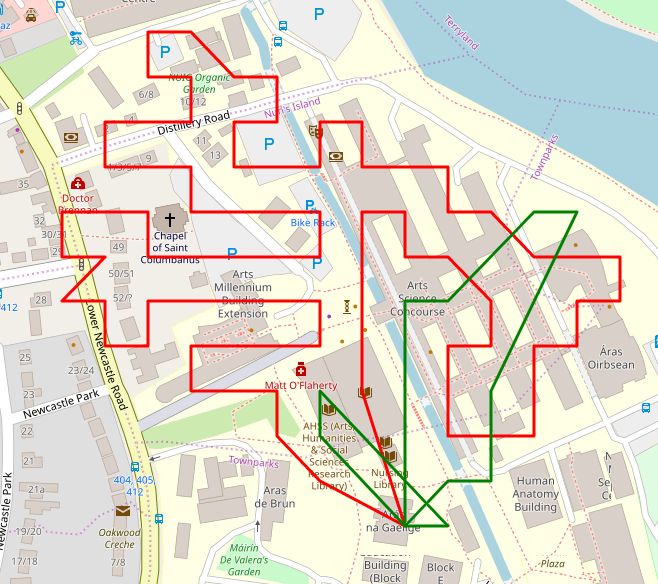
\includegraphics[width=\linewidth, height=51mm]{Chapters/MultiAgentCoverage/MultipleTravellingSalesman/Figs/ORToolsSolns/Example4.PNG}

    \end{minipage}
    &
    \small
    \begin{tabular}{m{10mm}|m{11mm} m{11mm}}
        & RAV 1 & RAV 2\\
        \hline
        Speed& 8 & 1 \\
        T.T.S & 1 & 1 \\
        Color & Red & Green \\
        \hline
        Dist.& 2638 & 870 \\
        Time& 1410 & 1600 \\
    \end{tabular}
    \normalsize
    \\
    \hline

  \end{tabular}
  \caption{Results of applying solution found with OR-Tools solver. T.T.S = Time to sample, Dist. = Distance}\label{table:ORToolsResults}
\end{table}
